\documentclass[11pt]{article}

  \usepackage{fullpage}
  \usepackage{graphicx}
  \graphicspath{ {./images/} }
  \setlength{\parindent}{0pt} 
  \setlength{\parskip}{1em}
  \begin{document}
  \title{ARM Final Report}
  \author{Otto White, Paulo Lemos, Robert Stok, Weizhong Zhao}

  \maketitle

  \section*{Assembler Structure and Implementation}

  \begin{figure}[h]
  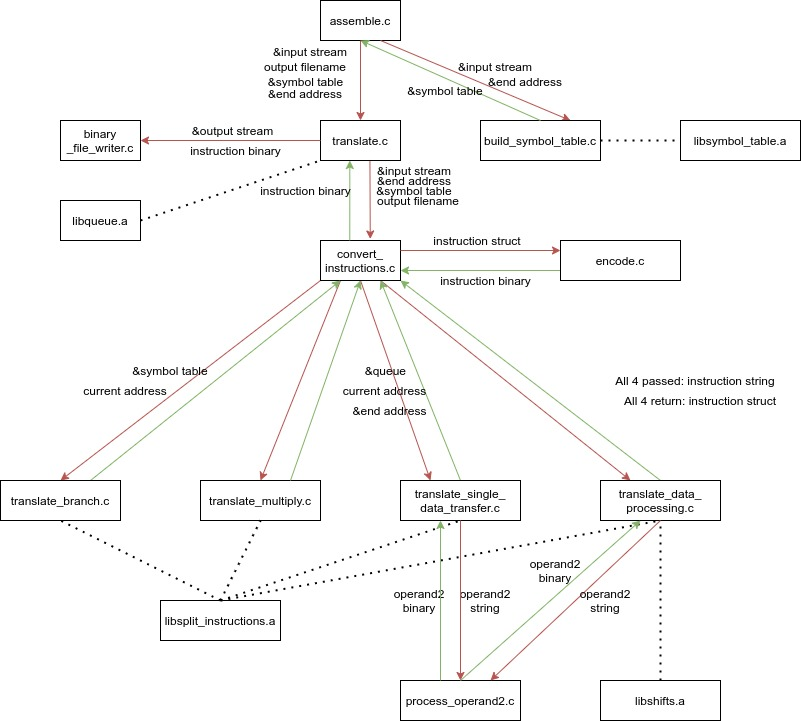
\includegraphics[scale=0.3]{assembler_structure}
  \centering
  \end{figure}

The assembler is structured as follows:

\begin{itemize}
\item \texttt{assemble.c} contains the main function which takes the input and output filenames as arguments; the input file contains ARM11 assembly instructions and the output file will have assembled ARM11 binary code written to it. Main calls build\_symbol\_table from \texttt{build\_symbol\_table.c} which passes through the input file once. After rewinding the input file to the original file position, translate from \texttt{translate.c} is called for the second pass. Finally, the memory allocated to symbol table is freed to prevent memory leaks.

\item \texttt{build\_symbol\_table.c} defines the build\_symbol\_table function which creates a node-based linked list mapping labels to memory addresses from label assignment instructions found in the input file. Each node struct has memory dynamically allocated and stores a label, an address and a pointer to the next node. Various helper functions and the struct definition are in symbol\_table.c in the \texttt{utilities} folder. In particular, the search\_table function is useful for retrieving the memory address when given a label. The head node is returned by build\_symbol\_table.

\item \texttt{translate.c} defines the translate function which reads the input file line by line. Next, each line is passed to convert\_instructions in \texttt{convert\_instructions.c} and then written to the output file with binary\_file\_writer in \texttt{utilities}.

\item \texttt{convert\_instructions.c} defines the convert\_instructions function. First, this determines the nature of an instruction and passes it to the appropiate function from translate\_multiply, translate\_single\_data\_transfer, translate\_branch or translate\_data\_processing. The output is then fed through encode in \texttt{encode.c} and returned.

\item \texttt{translate\_multiply.c, translate\_single\_data\_transfer.c, translate\_branch.c, and translate\_data\_processing.c} each define the respective translate functions. A common tokenizer in split\_instructions.c in \texttt{utilities} is used to seperate the instruction and avoid code duplication. A new Instruction struct, representing the instruction, is populated with relevant opcodes and operand fields and then returned.

\item \texttt{encode.c} defines the encode function which builds the final binary word from the instruction struct and returns it as a uint\_32t.

\item \texttt{definitions.h} contains the Instruction\_Type, Condition and Opcode enum and Instruction struct definitions.

\item \texttt{utilities} contains binary\_file\_writer, split\_instructions(tokenizer), symbol\_table and miscellaneous helper functions for specific instruction translation functions.

\item \texttt{testing} contains unit tests for different parts of the assembler.

We decided to implement a two pass assembler as . The idea of writing line by line

\end{itemize}

  \section*{Extension}

  \subsection*{}
  \subsection*{}
  \subsection*{}

  \section*{Evaluation}

  \subsection*{Group Reflection}

Communication was primarily carried out through online meetings and messaging throughout the project. Although this may have hindered group programming, we felt this medium was adequate for making design decisions, allocating work or helping each other solve problems. Meetings were held almost daily throughout the project and on days where we could not all meet, we kept each other updated on the progress of our work through messages. We also used a Gantt chart through Google Sheets which each member updated to track the progress of individual tasks; this gave a good visual representation of our progress but it was less frequently updated later on as we talked enough to know where everyone was at.

Our work allocation was generally fair and members were often assigned tasks they thought they would be stronger at to ensure a better outcome. At the beginning of all three tasks, we decided together the structure and the main functions we needed to implement before distributing work. This gave each member a better understanding of how their work integrated into the entire project as well as a broader view of the program.

In terms of things we would change, we feel that our group could be slightly more timely with finishing our tasks. There were times when a certain part would be a day late although this was not severely detrimental as we set our internal deadlines quite ambitiously. We could also adhere more closely to our decided code style standards as we faced some code style issues e.g bad variable names which made debugging more difficult. Another change could be more in-person group programming sessions which could be more efficient as communication would be more straightforward.

Our strengths for this project would be our consistency and organisation. Throughout the project, we have kept a steady tempo in finishing tasks in a way that we weren't rushed at the end. Our git organisation was also tidy as we used branches for individual tasks and kept to a standard commit style.

Overall, we feel we have worked well as a group with all members contributing fairly and achieving our objectives.

  \subsection*{Individual Reflection}

  \end{document}
